\documentclass{beamer}
\usepackage{times}
\usepackage[czech]{babel}
\usepackage[utf8]{inputenc}
% \usetheme{Berkeley}
% \usetheme{Copenhagen}
\usetheme{Madrid}
% \usecolortheme{beaver}
\newcommand{\czuv}[1]{\quotedblbase #1\textquotedblleft}
\usepackage{graphicx}
\usepackage{amsmath}
\setbeamertemplate{caption}[numbered]

\title{Výkresy}
\subtitle{Tvorba ER diagramu}
\author{Matějka Jiří a Míšová Miroslava}
\date{\today}
%\logo{\includegraphics[width=3cm]{FIT.eps}}

\begin{document}
  \frame{\titlepage}
%%%%%%%%%%%%%%%%%%%%%%%%%%%%%%%%%%%%%%%%%%%%
  \begin{frame}
    \frametitle{Obsah}

    \begin{itemize}
      \item Zadání
      \item Entitní množiny
      \item Položky entitních množin
      \item Vztahy mezi entitními možinami
      \item Výsledný ER Diagram
    \end{itemize}
  \end{frame}
%%%%%%%%%%%%%%%%%%%%%%%%%%%%%%%%%%%%%%%%%%%%
  \begin{frame}
    \frametitle{Zadání - Výkresy}
    \hspace{2mm}
      \scriptsize{
      Předpokládejte, že analyzujete požadavky na systém, který bude poskytovat počítačovou
      podporu pro kreslení stavebních výkresů. Z informací, které máte dosud k dispozici,
      vyplývá, že jednotkou, se kterou bude systém pracovat, bude výkres. Každý výkres bude
      mít svůj název, autora, datum poslední změny a řadu dalších atributů, a bude se týkat
      nemovitosti, u níž ukládáme název a místo.\par


      \hspace{0.5cm}Pro jednu nemovitost může existovat více výkresů. Výkres obsahuje jednu nebo více tzv.
      vrstev (např. vrstva s půdorysem budovy, rozvody plynu, elektřiny apod.), do nichž se
      umísťují geometrické útvary. Na jedné vrstvě se může nacházet řada geometrických útvarů,
      ale každý z nich je vždy jen na jedné vrstvě. Každá vrstva má své jednoznačné jméno.\par


      \hspace{0.5cm}Geometrické útvary lze rozdělit do dvou skupin -- primitivní a složené. Jako primitivní
      uvažujte bod, lomenou čáru a uzavřenou oblast. Složené útvary vznikají seskupením jiných
      útvarů (primitivních i složených). Protože musí být k dispozici i operace, která rozloží
      složený útvar na útvary, jejichž seskupením vznikl, musí být tato informace (tj. které
      prvky seskupení tvoří) k dispozici. Jedním z dalších požadavků je, aby systém pracoval
      s určitými rozšířitelnými paletami -- barev, typů čar a typů výplně. Každá vrstva má
      potom definovanou implicitní barvu (jedna barva  z  palety) a barvu podkladu, každý
      primitivní prvek může mít definovánu jinou barvu (opět z palety). Podobně lomená čára
      a uzavřená oblast mají definován typ čáry a uzavřená oblast navíc typ výplně – opět
      z příslušných palet.\par}

  \end{frame}
%%%%%%%%%%%%%%%%%%%%%%%%%%%%%%%%%%%%%%%%%%%%
  \begin{frame}
    \frametitle{Entitní množiny}
      \scriptsize{
      \hspace{0.5cm}Předpokládejte, že analyzujete požadavky na systém, který bude poskytovat počítačovou
      podporu pro kreslení stavebních výkresů. Z informací, které máte dosud k dispozici,
      vyplývá, že jednotkou, se kterou bude systém pracovat, bude \textcolor{blue}{výkres}. Každý výkres bude
      mít svůj název, autora, datum poslední změny a řadu dalších atributů, a bude se týkat
      \textcolor{blue}{nemovitosti}, u níž ukládáme název a místo.\par


      \hspace{0.5cm}Pro jednu nemovitost může existovat více výkresů. Výkres obsahuje jednu nebo více tzv.
      \textcolor{blue}{vrstev} (např. vrstva s půdorysem budovy, rozvody plynu, elektřiny apod.), do nichž se
      umísťují geometrické útvary. Na jedné vrstvě se může nacházet řada \textcolor{blue}{geometrických útvarů},
      ale každý z nich je vždy jen na jedné vrstvě. Každá vrstva má své jednoznačné jméno.\par


      \hspace{0.5cm}Geometrické útvary lze rozdělit do dvou skupin -- \textcolor{blue}{primitivní} a \textcolor{blue}{složené}. Jako primitivní
      uvažujte bod, lomenou čáru a uzavřenou oblast. Složené útvary vznikají seskupením jiných
      útvarů (primitivních i složených). Protože musí být k dispozici i operace, která rozloží
      složený útvar na útvary, jejichž seskupením vznikl, musí být tato informace (tj. které
      prvky seskupení tvoří) k dispozici. Jedním z dalších požadavků je, aby systém pracoval
      s určitými rozšířitelnými paletami -- barev, typů čar a typů výplně. Každá vrstva má
      potom definovanou implicitní \textcolor{blue}{barvu} (jedna barva  z  palety) a barvu podkladu, každý
      primitivní prvek může mít definovánu jinou barvu (opět z palety). Podobně lomená čára
      a uzavřená oblast mají definován typ čáry a uzavřená oblast navíc typ výplně – opět
      z příslušných palet.\par}
  \end{frame}
%%%%%%%%%%%%%%%%%%%%%%%%%%%%%%%%%%%%%%%%%%%%%
{
{
\usebackgroundtemplate{\centerline{$\vcenter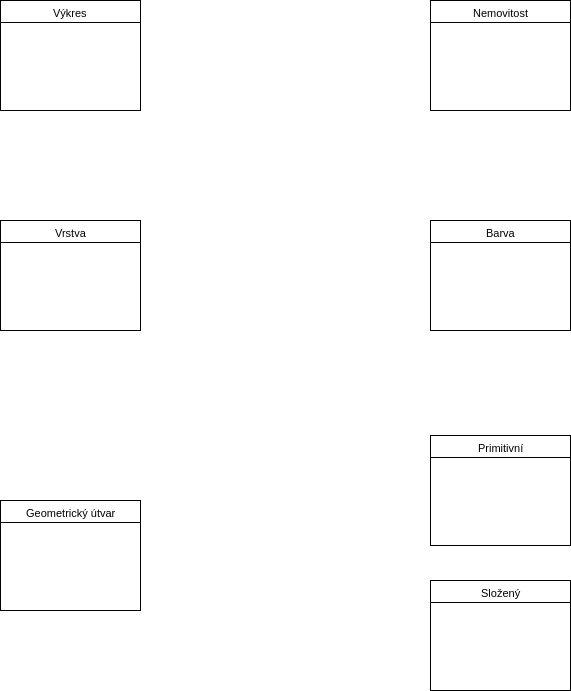
\includegraphics[height=0.8\paperheight]{prezentace1.png}$}}
\begin{frame}[plain]
\end{frame}
}
%%%%%%%%%%%%%%%%%%%%%%%%%%%%%%%%%%%%%%%%%%%%%
  \begin{frame}
    \frametitle{Položky entitních množin}
    \scriptsize{
    \hspace{0.5cm}Předpokládejte, že analyzujete požadavky na systém, který bude poskytovat počítačovou
    podporu pro kreslení stavebních výkresů. Z informací, které máte dosud k dispozici,
    vyplývá, že jednotkou, se kterou bude systém pracovat, bude \textcolor{blue}{výkres}. Každý výkres bude
    mít svůj \textcolor{red}{název, autora, datum poslední změny} a řadu dalších atributů, a bude se týkat
    \textcolor{blue}{nemovitosti}, u níž ukládáme \textcolor{red}{název a místo}.\par


    \hspace{0.5cm}Pro jednu nemovitost může existovat více výkresů. Výkres obsahuje jednu nebo více tzv.
    \textcolor{blue}{vrstev} \textcolor{red}({např. vrstva s půdorysem budovy, rozvody plynu, elektřiny apod.)}, do nichž se
    umísťují geometrické útvary. Na jedné vrstvě se může nacházet řada \textcolor{blue}{geometrických útvarů},
    ale každý z nich je vždy jen na jedné vrstvě. Každá vrstva má své \textcolor{red}{jednoznačné jméno}.\par


    \hspace{0.5cm}Geometrické útvary lze rozdělit do dvou skupin -- \textcolor{blue}{primitivní} a \textcolor{blue}{složené}. Jako primitivní
    uvažujte \textcolor{red}{bod, lomenou čáru a uzavřenou oblast}. Složené útvary vznikají seskupením jiných
    útvarů (primitivních i složených). Protože musí být k dispozici i operace, která rozloží
    složený útvar na útvary, jejichž seskupením vznikl, musí být tato informace (tj. které
    prvky seskupení tvoří) k dispozici. Jedním z dalších požadavků je, aby systém pracoval
    s určitými rozšířitelnými \textcolor{blue}{paletami} -- barev, typů čar a typů výplně. Každá vrstva má
    potom definovanou \textcolor{red}{implicitní barvu} (jedna barva  z  palety) a barvu podkladu, každý
    primitivní prvek může mít definovánu jinou barvu (opět z palety). Podobně lomená čára
    a uzavřená oblast mají definován typ čáry a uzavřená oblast navíc typ výplně – opět
    z příslušných palet.\par}
  \end{frame}
%%%%%%%%%%%%%%%%%%%%%%%%%%%%%%%%%%%%%%%%%%%%%%%%
{
{
\usebackgroundtemplate{\centerline{$\vcenter\includegraphics[height=0.8\paperheight]{prezentace2.png}$}}
\begin{frame}[plain]
\end{frame}
}
%%%%%%%%%%%%%%%%%%%%%%%%%%%%%%%%%%%%%%%%%%%%%
  \begin{frame}
      \frametitle{Vztahy entitních množin}
      \scriptsize{
      \hspace{0.5cm}Předpokládejte, že analyzujete požadavky na systém, který bude poskytovat počítačovou
      podporu pro kreslení stavebních výkresů. Z informací, které máte dosud k dispozici,
      vyplývá, že jednotkou, se kterou bude systém pracovat, bude \textcolor{blue}{výkres}. Každý výkres bude
      mít svůj název, autora, datum poslední změny a řadu dalších atributů, a \textcolor{orange}{bude se týkat}
      \textcolor{blue}{nemovitosti}, u níž ukládáme název a místo.\par


      \hspace{0.5cm}\textcolor{orange}{Pro jednu nemovitost může existovat více výkresů}. \textcolor{orange}{Výkres obsahuje jednu nebo více tzv.}
      \textcolor{blue}{vrstev} (např. vrstva s půdorysem budovy, rozvody plynu, elektřiny apod.), do nichž se
      umísťují geometrické útvary. \textcolor{orange}{Na jedné vrstvě se může nacházet řada \textcolor{blue}{geometrických útvarů},
      ale každý z nich je vždy jen na jedné vrstvě}. Každá vrstva má své jednoznačné jméno.\par


      \hspace{0.5cm}\textcolor{orange}{Geometrické útvary lze rozdělit do dvou skupin -- \textcolor{blue}{primitivní} a \textcolor{blue}{složené}}. Jako primitivní
      uvažujte bod, lomenou čáru a uzavřenou oblast. \textcolor{orange}{Složené útvary vznikají seskupením jiných
      útvarů (primitivních i složených)}. Protože musí být k dispozici i operace, která rozloží
      složený útvar na útvary, jejichž seskupením vznikl, \textcolor{orange}{musí být tato informace (tj. které
      prvky seskupení tvoří) k dispozici}. Jedním z dalších požadavků je, aby systém pracoval
      s určitými rozšířitelnými paletami -- barev, typů čar a typů výplně. Každá \textcolor{orange}{vrstva má
      potom definovanou implicitní \textcolor{blue}{barvu} (jedna barva  z  palety) a barvu podkladu}, \textcolor{orange}{každý
      primitivní prvek může mít definovánu jinou barvu} (opět z palety). Podobně lomená čára
      a uzavřená oblast mají definován typ čáry a uzavřená oblast navíc typ výplně – opět
      z příslušných palet.\par}
  \end{frame}
%%%%%%%%%%%%%%%%%%%%%%%%%%%%%%%%%%%%%%%%%%%%%%%%%%%
{
{
\usebackgroundtemplate{\centerline{$\vcenter\includegraphics[height=0.8\paperheight]{prezentace3.png}$}}
\begin{frame}[plain]
\end{frame}
}
%%%%%%%%%%%%%%%%%%%%%%%%%%%%%%%%%%%%%%%%%%%%%
  \begin{frame}
    \frametitle{Závěr}
    \begin{center}
      Děkujeme za pozornost
    \end{center}
  \end{frame}
\end{document}
